\chapter{Deploy dell'applicazione}
\label{cap:deploy}
\section{Scopo del capitolo}
Al termine dell'attività di stage, insieme al tutor, ho potuto osservare come avviene il deploy di una Spring Boot app su Docker.\\
Per deployment del software si intende la distribuzione o avviamento, con relativa installazione e configurazione, di un'applicazione. È considerabile come fase finale del ciclo di vita di un software, fase che conclude lo sviluppo e il collaudo, dando inizio alla manutenzione.
\section{Deploy}
\subsection{Dockerfile}
Per cominciare è stato creato un \texttt{Dockerfile} nella root del progetto. Questo file definirà come Docker dovrebbe costruire l'immagine.
\begin{figure}[H] 
    \centering 
    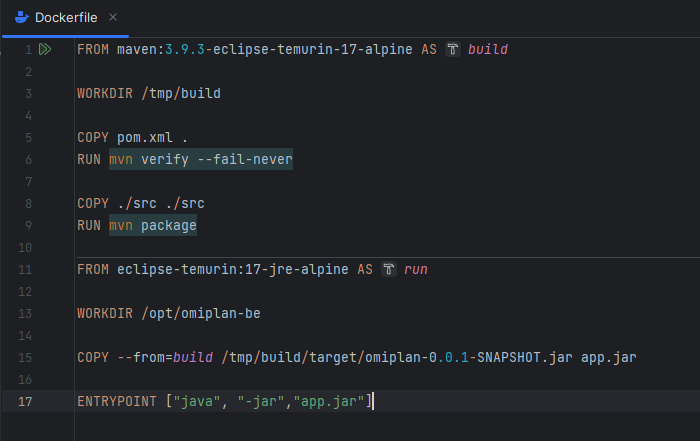
\includegraphics[width=0.80\columnwidth]{dockerfile} 
    \caption{Configurazione Dockerfile}
\end{figure}
\noindent All'interno del file, possiamo notare due sezioni separate, quella di build e quella di run (esecuzione).
\subsubsection*{Sezione Build}
Nella sezione di "build" viene indicato che si sta costruendo un'immagine di Docker basata su Maven 3.9.3 e Java 17. Vengono poi eseguite operazioni relative alla compilazione dell'applicazione, come la copia del file sorgente, la verifica delle dipendenze tramite il tool di build Maven e la crazione del pacchetto \texttt{.jar}.
\subsubsection*{Sezione Run}
La sezione di "run" ha come obiettivo l'esecuzione dell'applicazione. In questa sezione viene utilizzata nuovamente la stessa immagine di Java e vengono copiati i risultati della prima fase. L'istruzione finale \texttt{ENTRYPOINT} definisce il comando che verrà eseguito quando il container basato su questa immagine verrà avviato.
\subsection{Costruzione dell'immagine e avvio dell'applicazione}
In seguito alla creazione del \texttt{Dockerfile} si apre il terminale nella directory in cui si trova questo file.\\
Seguono poi i seguenti passi:
\begin{enumerate}
\item viene eseguito il comando \texttt{docker build -t nome\_immagine} per creare l'immagine Docker con le specifiche selezionate;
\item una volta costruita l'immagine si può avviare il container tramite il comando \texttt{docker run -ti nome\_immagine}; 
\item per accedere all'applicazione è possibile utilizzare un browser digitando il seguente indirizzo per interagire con l'applicazione: \textit{http://localhost:porta\_scelta}.
\end{enumerate}




